\documentclass{article}

\usepackage{geometry}
\usepackage{amsmath}
\usepackage{graphicx}
\usepackage{listings}
\usepackage{hyperref}
\usepackage{multicol}
\usepackage{fancyhdr}
\pagestyle{fancy}
\hypersetup{ colorlinks=true, linkcolor=black, filecolor=magenta, urlcolor=cyan}
\geometry{ a4paper, total={170mm,257mm}, top=20mm, right=20mm, bottom=20mm, left=20mm}
\setlength{\parindent}{0pt}
\setlength{\parskip}{1em}
\renewcommand{\headrulewidth}{0pt}
\lhead{Competitive Programming - Arkavidia VI}
\fancyfoot[CE,CO]{\thepage}
\lstset{
    basicstyle=\ttfamily\small,
    columns=fixed,
    extendedchars=true,
    breaklines=true,
    tabsize=2,
    prebreak=\raisebox{0ex}[0ex][0ex]{\ensuremath{\hookleftarrow}},
    frame=none,
    showtabs=false,
    showspaces=false,
    showstringspaces=false,
    prebreak={},
    keywordstyle=\color[rgb]{0.627,0.126,0.941},
    commentstyle=\color[rgb]{0.133,0.545,0.133},
    stringstyle=\color[rgb]{01,0,0},
    captionpos=t,
    escapeinside={(\%}{\%)}
}

\begin{document}

\begin{center}
    \section*{Pabrik} % ganti judul soal

    \begin{tabular}{ | c c | }
        \hline
        Batas Waktu  & 1s \\    % jangan lupa ganti time limit
        Batas Memori & 128MB \\  % jangan lupa ganti memory limit
        \hline
    \end{tabular}
\end{center}

\subsection*{Deskripsi}

Pak Joni adalah seorang insinyur dan pengusaha teknologi. Dia berniat untuk membangun suatu perusahaan mobil listrik di negara Arkavland.
Arkavland memiliki $N$ buah kota yang diberi nomor dari $1$ hingga $N$. Kota - kota tersebut dihubungkan dengan $M$ buah jalan dengan aturan sebagai berikut :

\begin{enumerate}
    \setlength\itemsep{0pt}
    \item Tiap jalan yang menghubungkan kota $A$ dan $B$ memiliki panjang $1$ km
    \item Jalanan di Arkavland adalah dua arah, artinya apabila terdapat jalan yang menghubungkan kota $A$ ke kota $B$ maka seseorang dapat berpindah dari kota $B$ ke kota $A$ juga
    \item Setiap pasang kota ($A$, $B$) di Arkavland akan terhubung dengan sebuah rute perjalanan tertentu
    
\end{enumerate}

Pak Joni ingin mobil listriknya dapat terdistribusi dengan mudah ke seluruh kota di Arkavland. Maka dibutuhkan keputusan ekonomi untuk menentukan kota mana yang paling optimal sebagai tempat dibangunnya pabrik mobil listrik tersebut. Bantulah pak Joni mencari kota di negara Arkavland yang memiliki jumlah jarak rute terpendek dari kota tersebut ke setiap kota lain dengan nilai yang paling minimum.

\subsection*{Format Masukan}
Baris pertama terdiri dari dua buah bilangan $N$ dan $M$ ($1 \leq M < N \leq 10^{6}$). $N$ dan $M$ berturut-turut menyatakan banyaknya kota dan jalan di negara Arkavland.
Baris kedua hingga baris ke $M + 1$ terdiri dari dua buah bilangan $A_i$ dan $B_i$ ($1 \leq $A_i$,$B_i$ \leq N$) yang menyatakan kota $A$ dan kota $B$ terhubung oleh jalan ke-$i$

\subsection*{Format Keluaran}
Sebuah baris berisi dua bilangan $A$ dan $X$. $A$ menyatakan nomor kota yang memiliki total jumlah jarak rute dari setiap kota lain ke kota tersebut adalah yang paling minimum dan $X$ menyatakan total jumlah jaraknya. Jika terdapat banyak solusi, keluarkan jawaban dengan nomor kota yang paling kecil.
\\

\begin{multicols}{2}
\subsection*{Contoh Masukan}
\begin{lstlisting}
4 3
1 2
2 3
3 4
\end{lstlisting}
\columnbreak
\subsection*{Contoh Keluaran}
\begin{lstlisting}
2 4
\end{lstlisting}
\vfill
\null
\end{multicols}

% \subsection*{Penjelasan}

% 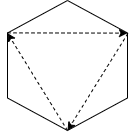
\includegraphics[width=40px]{1.png}
% 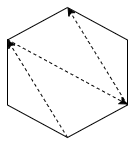
\includegraphics[width=40px]{2.png}
% 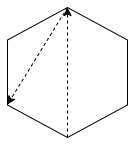
\includegraphics[width=40px]{3.png}
% 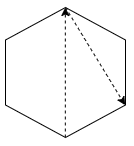
\includegraphics[width=40px]{4.png}
% 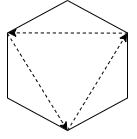
\includegraphics[width=40px]{5.png}
% 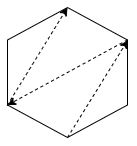
\includegraphics[width=40px]{6.png}


\pagebreak

\end{document}